\chapter{But du travail}

%\section{Explication du projet eSWARM}

Ce stage s'inscrit dans la continuité du projet eSWARM et poursuit les travaux d'Augustin Bonnel~\cite{bonnel_modeling_2024} et de Sylvain Boegeat, deux anciens étudiants de l'INSA\@. L'objectif de ce projet est de développer un système de drones quadricoptères modulaire et reconfigurable, capable de s'assembler en vol afin d'accomplir des missions qu'un drone seul ne pourrait réaliser, comme par exemple le transport de charges lourdes.

Le projet eSWARM est basé sur des essaims de robots dits reconfigurables et modulaires. Une définition de ce type de système est donnée dans \cite{seo_modular_2019} : "Les systèmes de robots modulaires reconfigurables (\gls{mrr}) sont constitués de nombreux modules (ou unités) répétés qui peuvent être réorganisés dans différentes configurations en fonction de la tâche que le robot doit accomplir." Une définition similaire est fournie dans \cite{brooks_overview_2021}.
\begin{wrapfigure}{r}{0.35\textwidth}
    %\vspace{0.3cm} 
    \centering
    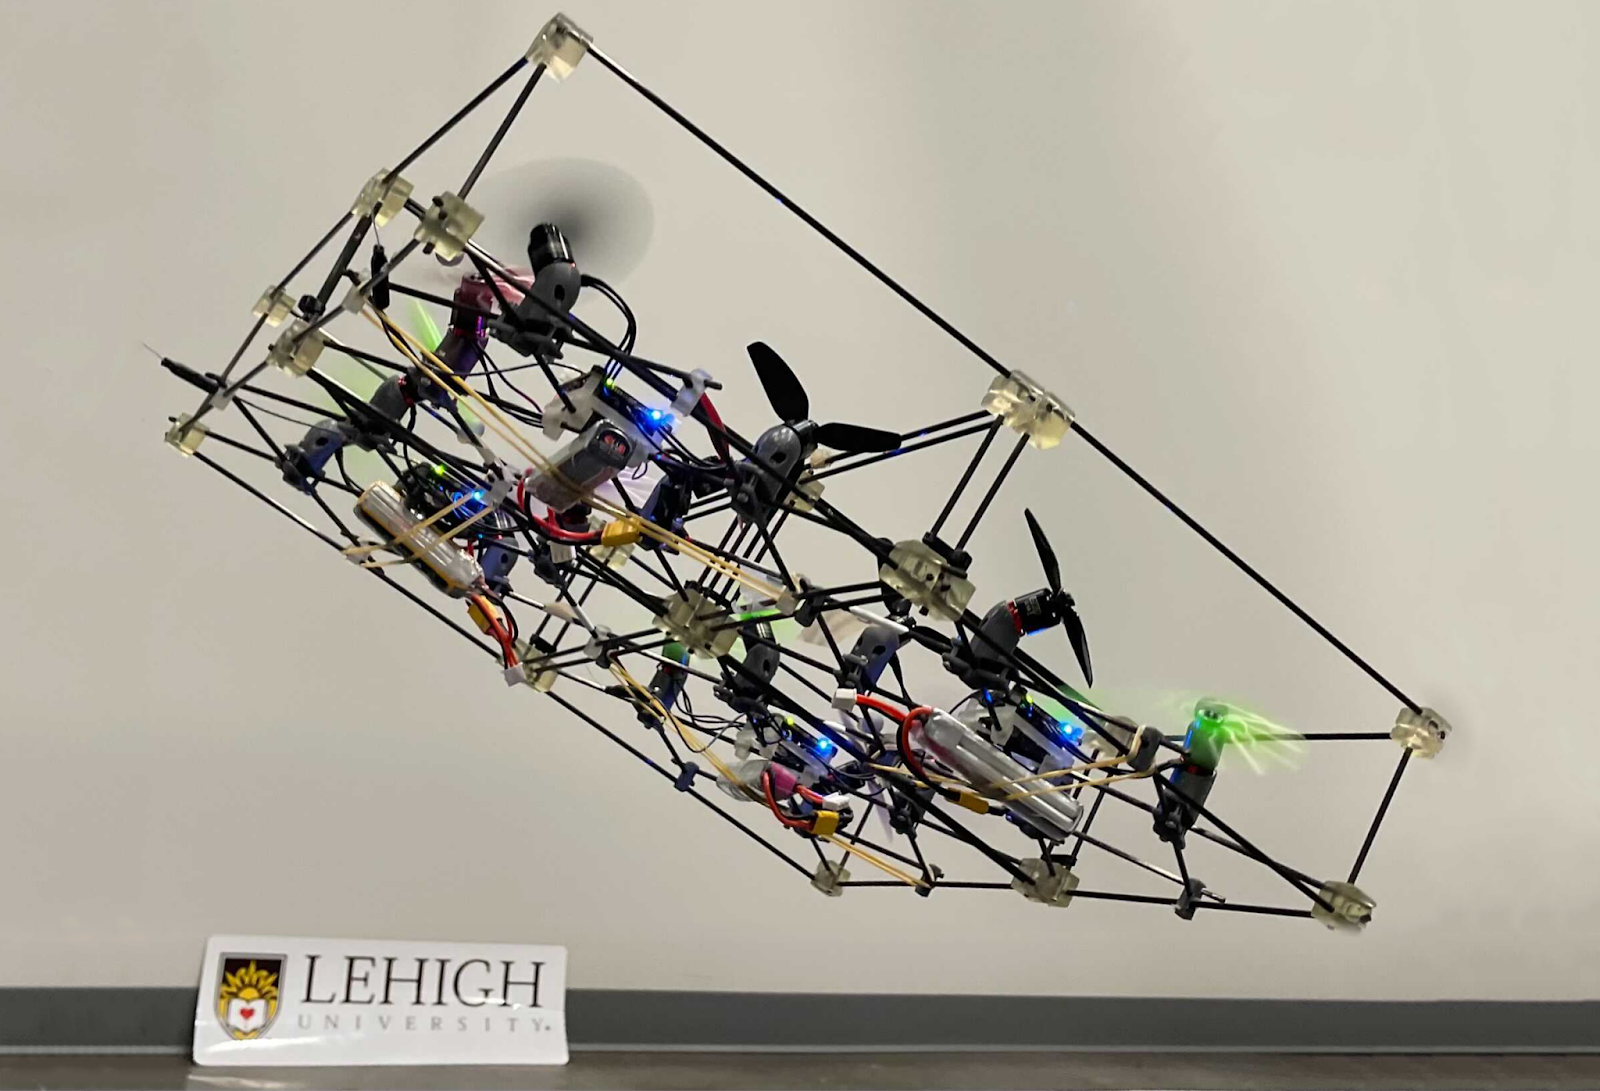
\includegraphics[width=0.3\textwidth]{6-But_du_travail/pic/modquad.png}
    \caption{Système ModQuad \cite{saldana_modquad_2018}.}
    \label{fig:Modquad2018}
    \vspace{-0.5cm} 
\end{wrapfigure}
Il est essentiel d'expliquer les deux termes : \textit{modulaire} et \textit{reconfigurable}. Le premier désigne une architecture composée de modules pouvant s'assembler de diverses manières. Le second caractérise la capacité du système à modifier sa structure au cours de son fonctionnement.


L'une des principales sources d'inspiration pour ce projet est le projet ModQuad \cite{saldana_modquad_2018}, qui est un système d'essaim modulaire reconfigurable de drones quadricoptères. Il est composé de modules qui peuvent s'assembler pour former des structures plus grandes et plus complexes. Un exemple est donné ci-contre (Figure \ref{fig:Modquad2018}). 
Globalement, le système peut être schématisé comme suit : 

\begin{figure}[htbp]
    \centering
    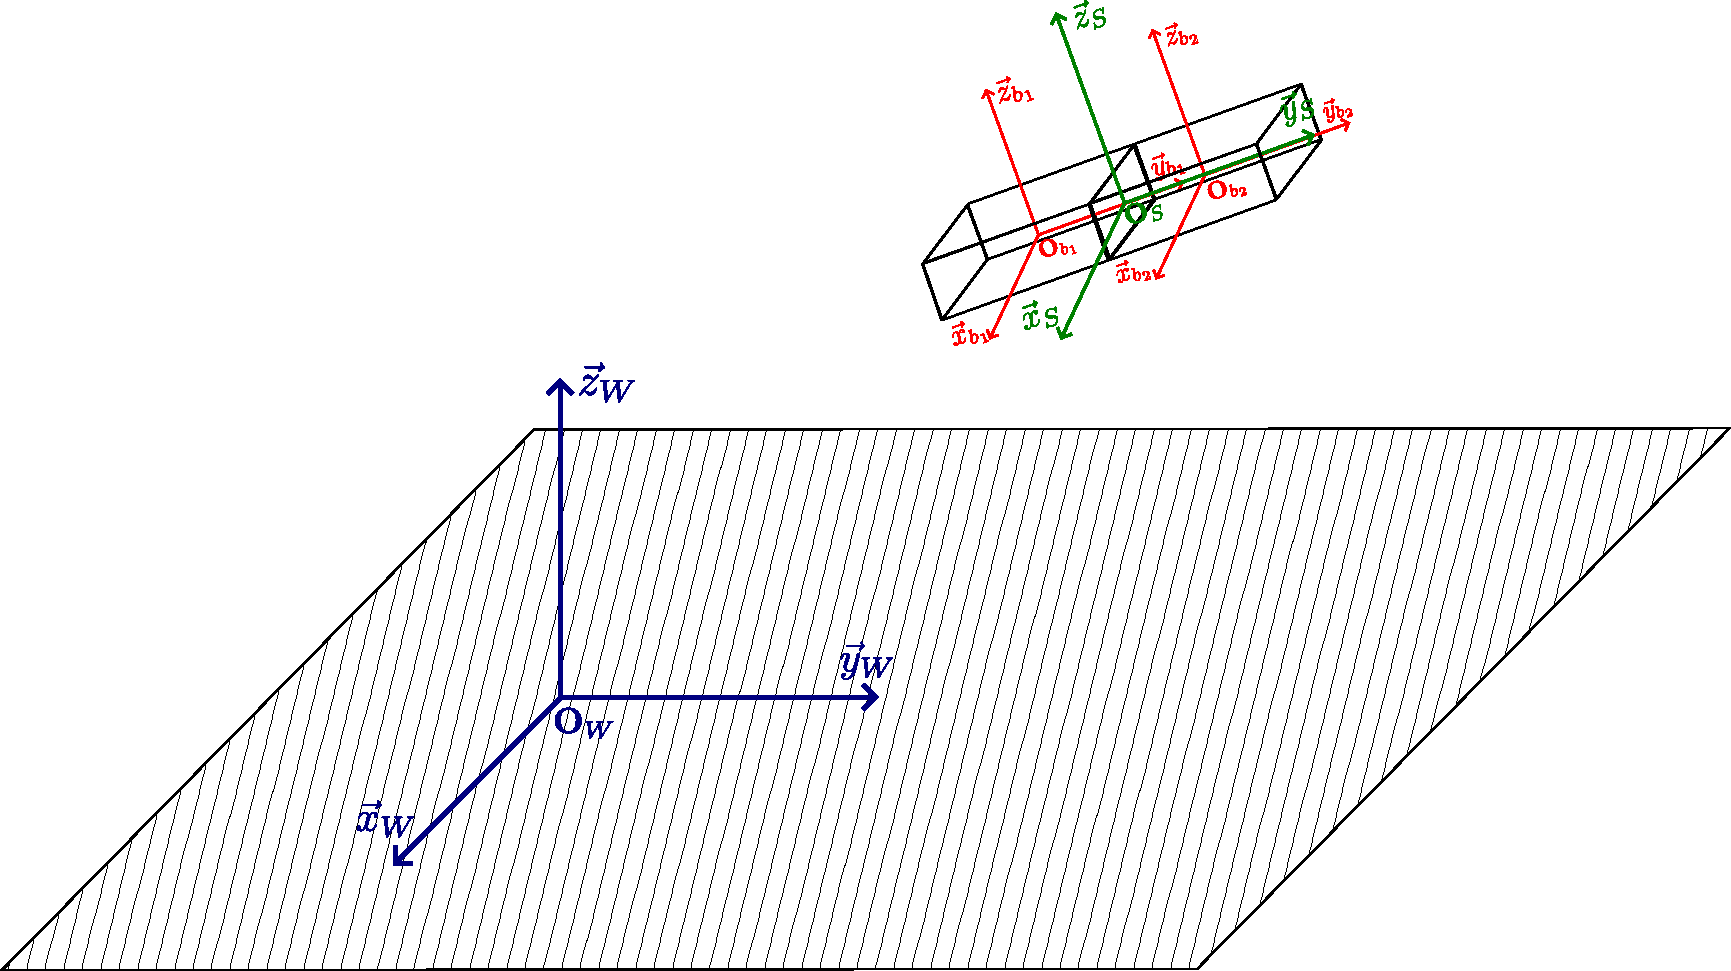
\includegraphics[width=0.85\linewidth]{6-But_du_travail/pic/structure_2drones_schema.pdf}
    \caption{Schéma global du système. \cite{bonnel_modeling_2024}}
    \label{fig:schema_systeme}
\end{figure}

Il y a deux quadricoptères, représentés par les repères rouges $O_{bi}$ attachés ensemble. L'objectif est donc de développer la loi de commande permettant de piloter cette structure (repère $O_S$). Avec deux drones, il n'y a qu'une seule configuration possible, mais plus le nombre de drones augmente, plus le nombre de configurations possibles croît rapidement. Il s'agit donc de développer une méthode de calcul de commande pouvant s'adapter à n'importe quelle configuration.


%\begin{figure}[h]
%    \centering
%    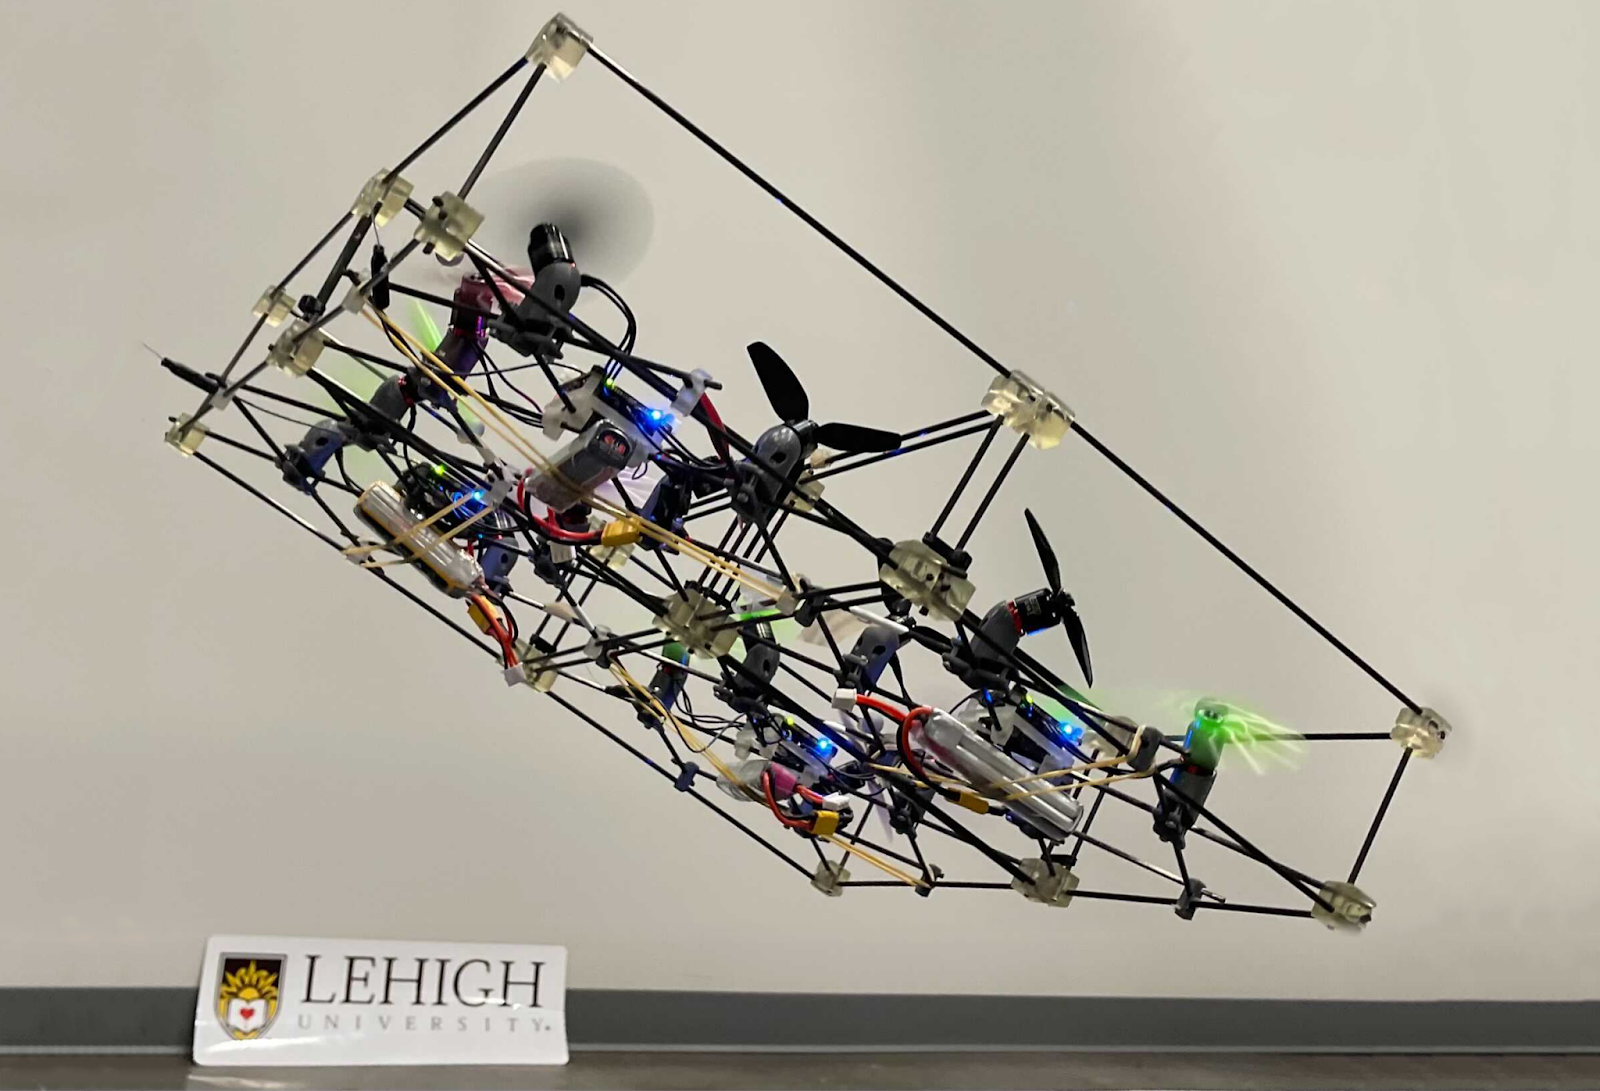
\includegraphics[width=0.5\textwidth]{6-But_du_travail/pic/modquad.png}
%    \caption{Système ModQuad \cite{saldana_modquad_2018}.}
%    \label{fig:Modquad2018}
%\end{figure}

Pour le stage, il a été décidé de remplacer les drones par des robots terrestres holonomes. Bien que le projet eSWARM soit initialement axé sur les drones aériens, leur utilisation implique des contraintes techniques : autonomie réduite (souvent inférieure à dix minutes) et les risques de crash et de casse de matériel ne sont pas négligeables. Cela peut ralentir le déroulement des expérimentations. Les robots utilisés sont montrés ci-dessous (Figure \ref{fig:essaim}).
\begin{figure}[htbp]
    \centering
    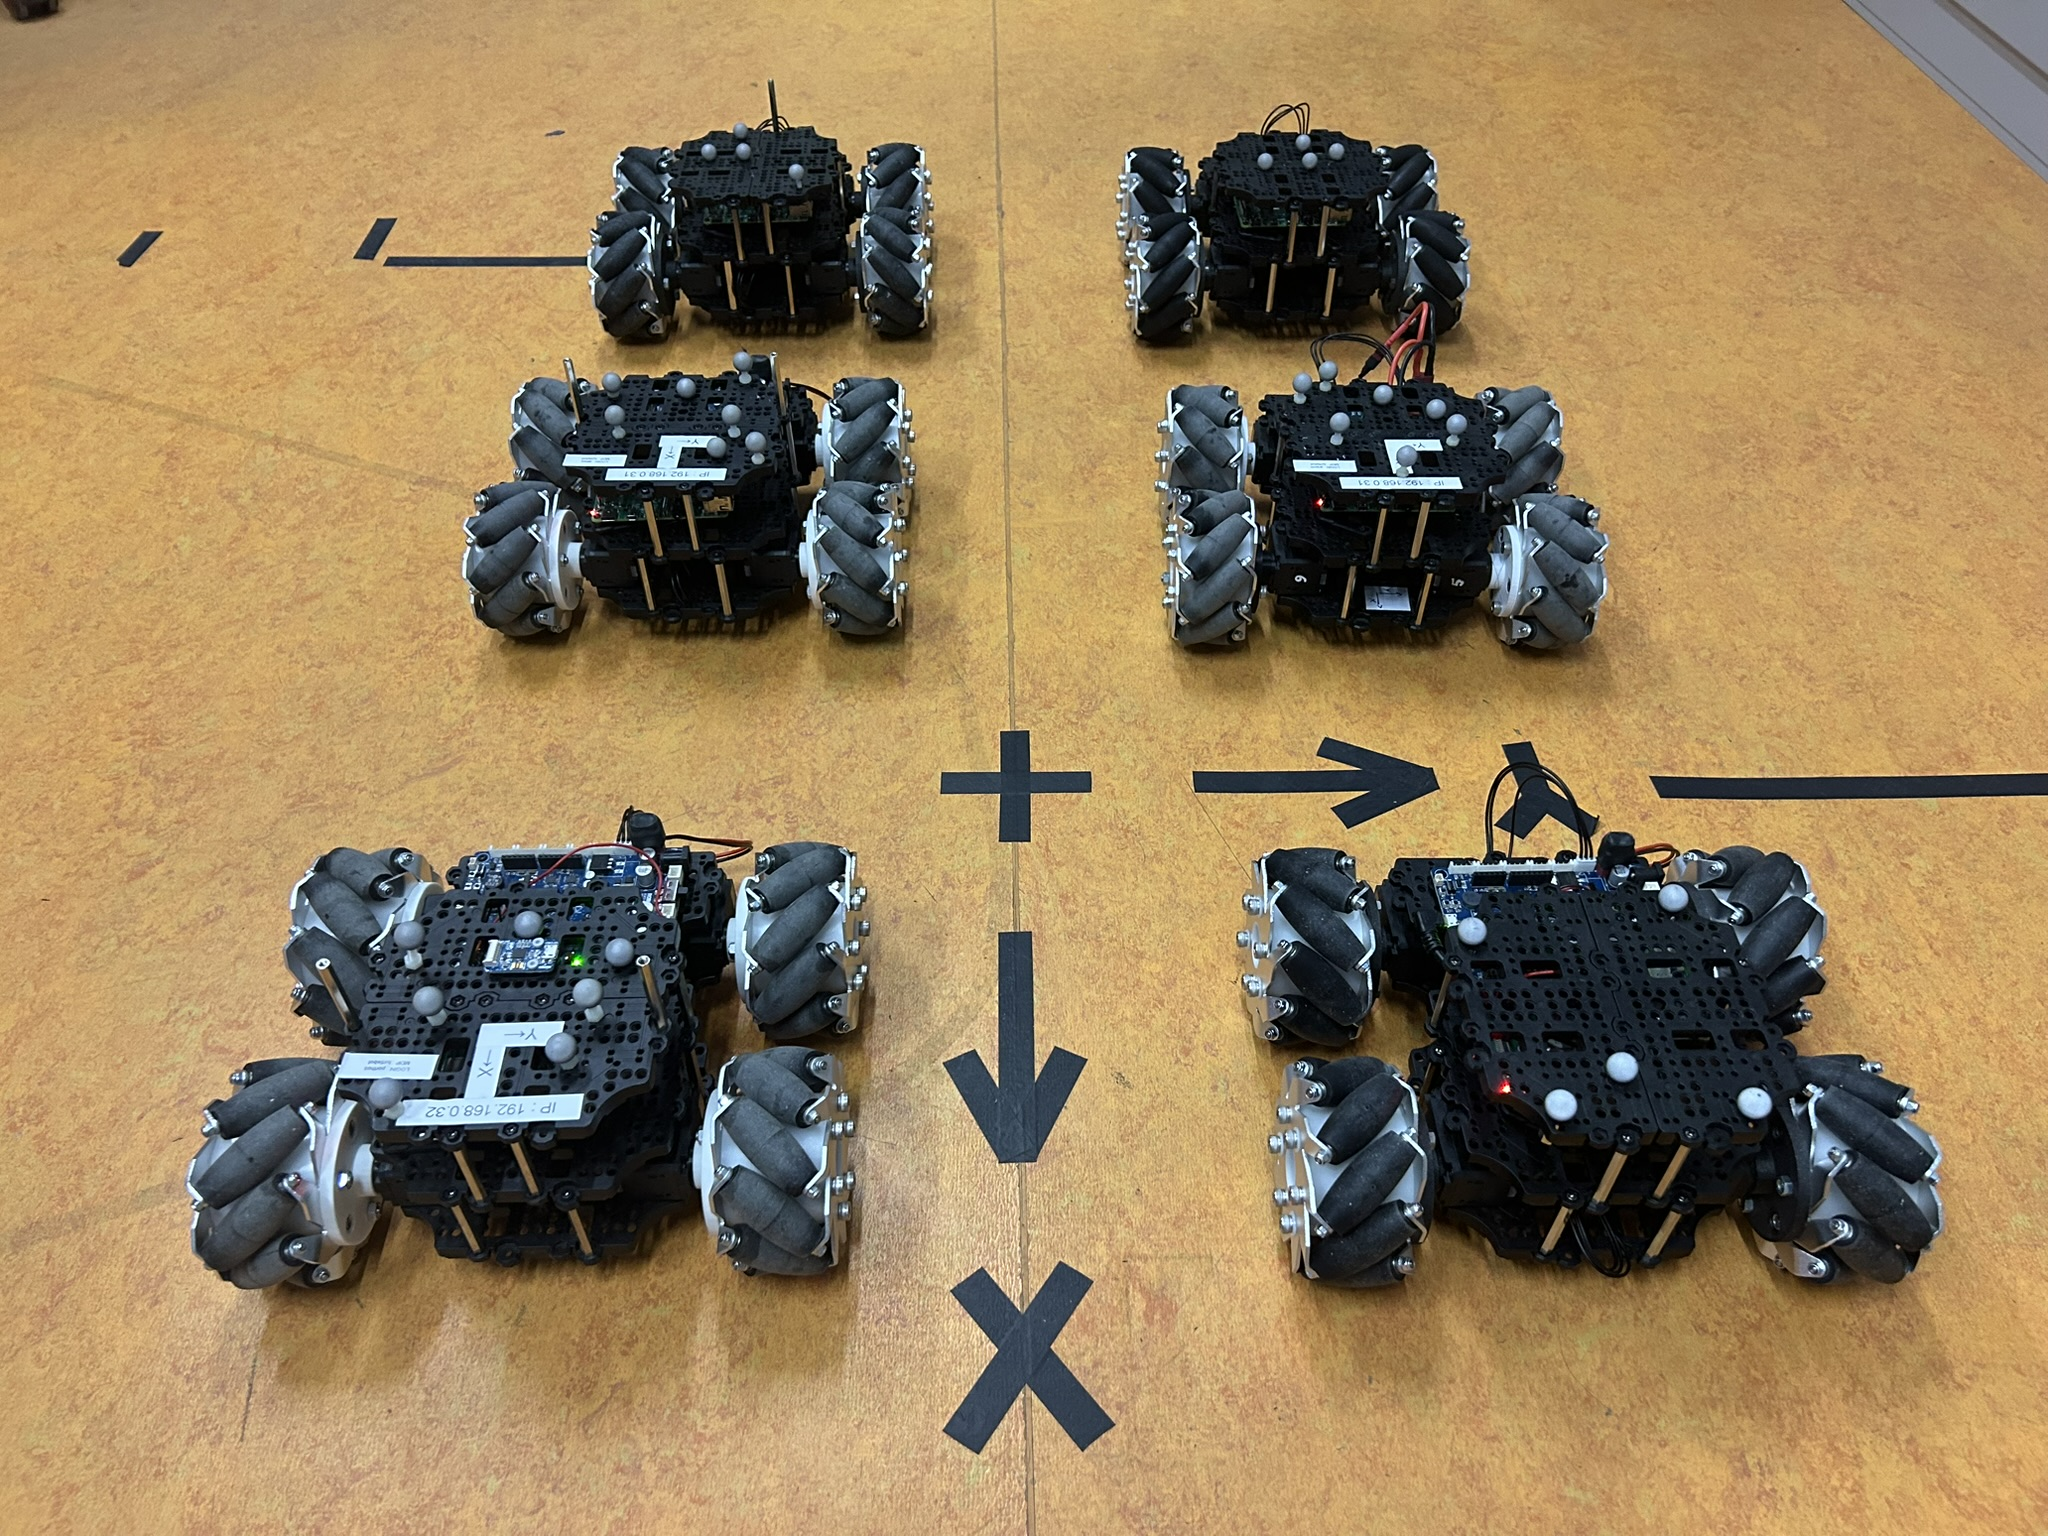
\includegraphics[width=0.7\linewidth]{6-But_du_travail/pic/essaim.JPEG}
    \caption{Essaim de robots terrestres holonomes utilisé pour les expérimentations.}
    \label{fig:essaim}
\end{figure}

L’un des objectifs de ce stage est aussi l’optimisation des lois de commande dans ce contexte d'essaim de robots. Il s’agit de concevoir une commande distribuée permettant de piloter efficacement la formation de l’essaim, tout en assurant sa stabilité, sa réactivité et sa robustesse.

%\section{Nature du travail et cahier des charges}

Les travaux menés au cours du stage porteront donc dans un premier temps sur le développement d'une plateforme de robots terrestres holonomes remplaçant la plateforme drone initiale, afin de simplifier les expérimentations. La seconde étape sera le développement logiciel d'une architecture distribuée (ROS2) permettant la gestion d'un essaim de robots. Enfin, la dernière étape sera l'optimisation de la commande distribuée pour l'essaim de robots, par l'implémentation de paradigmes de contrôle événementiel.

%\section{Dimension recherche}

La partie recherche porte sur les questions suivantes : comment garder une formation stable avec peu d'échanges réseau, quel est l'effet des perturbations sur la convergence, et quel compromis trouver entre réactivité et consommation. L'approche consiste à implémenter différentes méthodes de commande événementielle, puis à injecter des perturbations (panne simulée, retard de communication) pour mesurer robustesse, temps de convergence et erreur finale. Les résultats attendus sont un jeu de mesures comparatives, et une base à transférer ensuite vers la version aérienne du projet.

